% @Author: AnthonyKenny98
% @Date:   2020-02-23 14:26:30
% @Last Modified by:   AnthonyKenny98
% @Last Modified time: 2020-04-10 10:22:28



    \subsection{RISC-V}
    \subsubsection{Extending RISC-V}
    RISC-V is designed cleverly in a modular way, with a set of base instruction sets and a set of standard extensions. As a result, processors can be designed to only implement the instruction groups it requires, saving time, space and power on instructions that won't be used. In addition, another goal of RISC-V is to provide a basis for more specialized instruction-set extensions or more customized accelerators. This is described in the most recent \textit{RISC-V Instruction Set Manual} \cite{Waterman2019}. This is a powerful feature, as it does not break any software compatability, but allows for designers to easily follow the steps outlined in Figure \ref{fig:extendingRISCV}. From a \gls{hardware acceleration} point of view, this is particularly useful as it allows the designer to directly invoke whatever functional unit or accelerator they implement from assembly code.
    % @Author: AnthonyKenny98
% @Date:   2020-03-01 10:28:34
% @Last Modified by:   AnthonyKenny98
% @Last Modified time: 2020-03-01 10:32:45
\begin{figure}[H]
\begin{center}
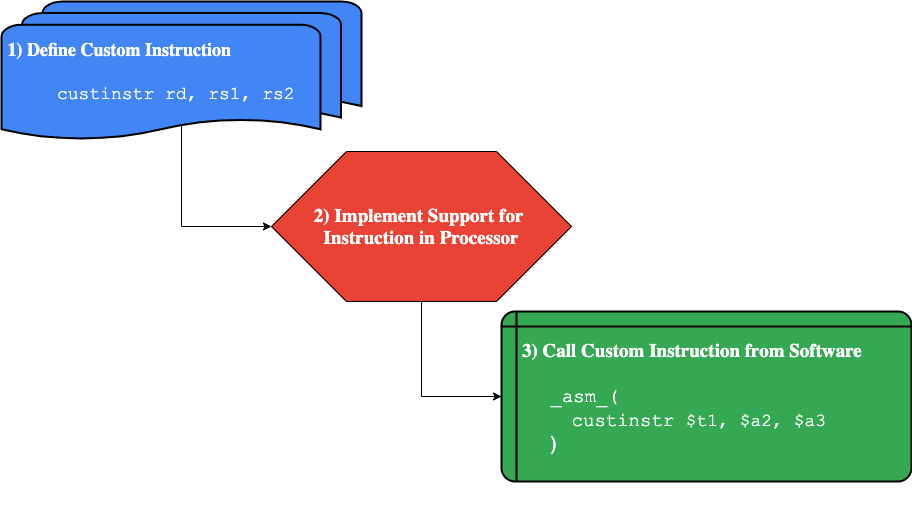
\includegraphics[width=0.9\linewidth]{chapters/chapter1/img/extendingRISCV.png}
\caption{Typical Process of Adding Non-Standard Extension to RISC-V ISA}
\label{fig:extendingRISCV}
\end{center}
\end{figure}

    \subsubsection{Accelerating RISC-V Processors}
    Having only been released in 2011, RISC-V is still a relatively unexplored opportunity for non-education applications. However, it shows promise in the commercial space, with Alibaba recently developing the Xuantie, a 16-core, 2.5GHz processor, currently the fastest RISC-V processor. Recently there has been promising research into accelerating computationally complex applications, particularly in edge-computing, with RISC-V architecture. \\
    \textit{Towards Deep Learning using TensorFlow Lite on RISC-V}, a paper co-written by the faculty advisor of this thesis, V.J. Reddi, presented the software infrastructure for optimizing the execution of neural network calculations by extending the RISC-V ISA and adding processor support for such extensions. A small number of instruction extensions achieved coverage over a wide variety of speech and vision application deep neural networks. Reddi et al. were able to achieve an 8 times speedup over a baseline implementation when using the extended instruction set.
    \textit{GAP-8: A RISC-V SoC for AI at the Edge of the IoT} proposed a programmable RISC-V computing engine with 8-core and convolutional neural network accelerator for power efficient, battery operated, IoT edge-device computing with order-of-magnitude performance improvements with greater energy efficiency. \\

